\begin{figure}
    \begin{small}
        \begin{center}
            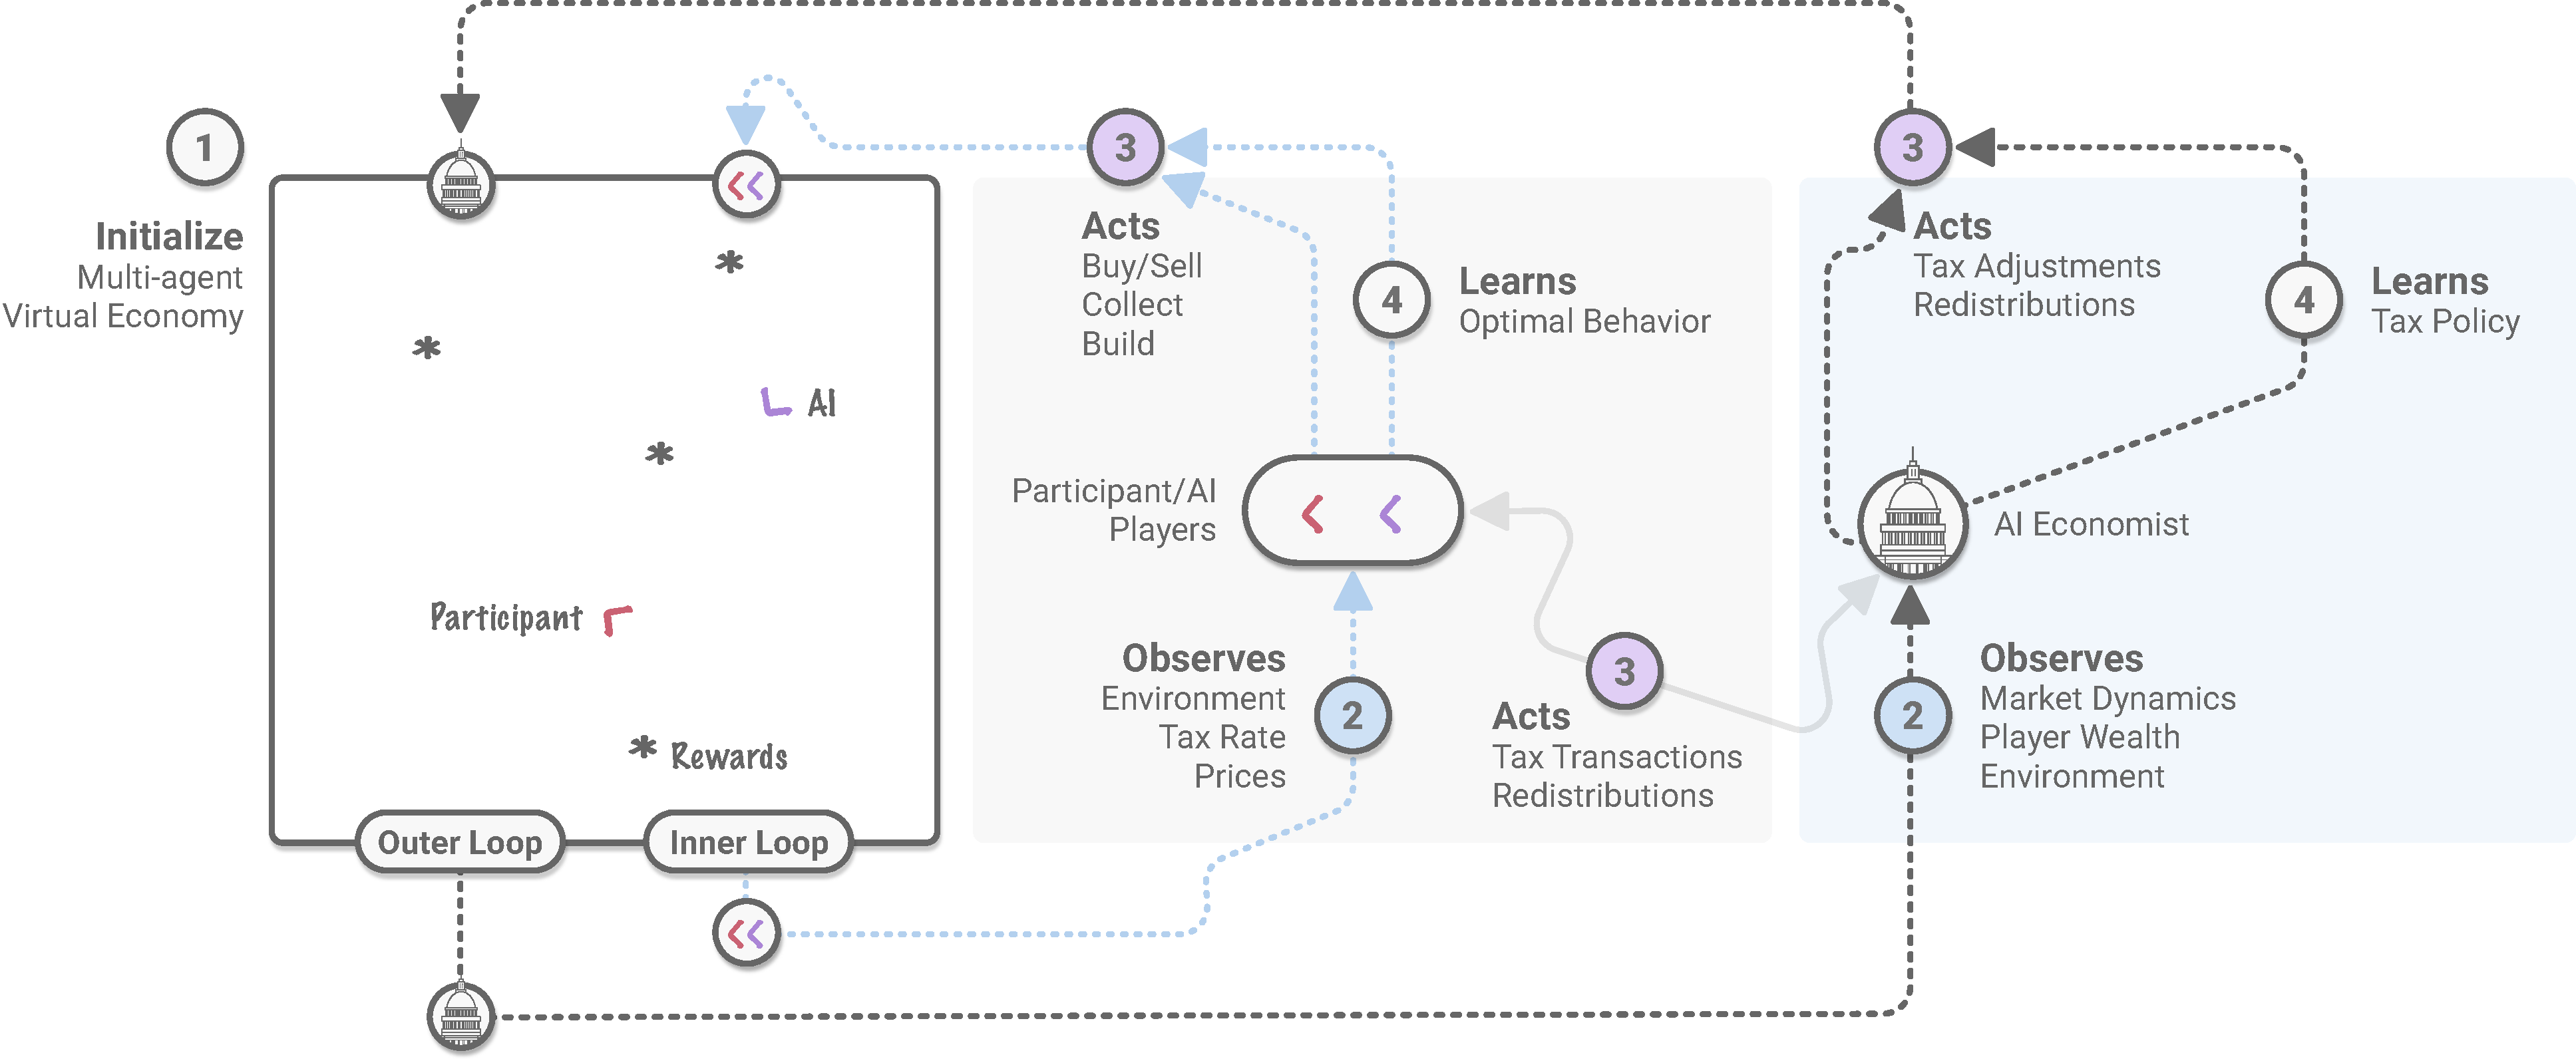
\includegraphics[width=0.95\textwidth]{figures/postprocessed/twolevelrl.pdf}
        \end{center}
        \caption{Two-level RL. In the inner loop, RL agents gain experience by performing labor, receiving income, and paying taxes, and learn through balancing exploration and exploitation how to adapt their behavior to maximize their utility. In the outer loop, the social planner adapts tax policies to optimize its social objective.}
        \label{fig:innerouterrl}
    \end{small}
\end{figure}
\subsection{Inner-Outer-Loop Reinforcement Learning}
\label{sect:innerouterrl}
Reinforcement learning provides a suitable learning framework for adapting behaviors in a sequential environment, and is used here to allow both the economic agents and the social planner to learn from experience collected through trial-and-error strategies. 
We conceptualize the RL framework used in this paper as including two levels of learning, namely an `inner' loop and an `outer' loop, as depicted in Figure~\ref{fig:innerouterrl}.

In short, the key benefits of our RL framework are:
\begin{itemize}
    \item the social planner can optimize taxes for any social objective \socialwelfare, and
    \item given a choice of social welfare functions $\socialwelfare$, the social planner does not need prior world knowledge, prior economic knowledge, or assumptions on the behavior of economic agents.
\end{itemize}

The main challenge posed by this two-level RL problem comes from the fact that each level effectively determines the MDP faced by the other level.
As the planner learns and changes taxes, the agents' utility and reward landscapes change.
In turn, as agents learn and adapt to new taxes, their behavior changes the expected social welfare generated through the tax schedule.
In this way, simultaneous learning creates an unstable reward landscape for both the  agents and the planner.
\paragraph{Inner Loop.}
In the inner loop, RL agents gain experience by performing labor, receiving income, and paying taxes, and learn through trial-and-error how to adapt their behavior to maximize their utility. Given a fixed tax policy, this is a standard RL problem in which agents iteratively explore and discover which behaviors are optimal for their fixed utility function, while observing the active tax schedule.

However, because the tax policy is changing, and in turn the behavior of others, the agent is faced with a non-stationary MDP.
Specifically, the utility of agent $i$ depends on its post-tax incomes $\endow_i$ (Eq \ref{eq:posttaxincome}).
The non-stationarity faced by agents can be understood by considering their learning objective in the context of a changing tax policy (generalizing Eq \ref{eq:agentproblem}):
\eq{\label{eq:agentproblemposttax}
    \max_{\policy_i}
    \E_{
    \ac_i    \sim \policy_i,
    \Ac_{-i} \sim \V{\policy}_{-i},
    \mtaxrate \sim \plannerpolicy,
    \st'\sim\trans
    }\brcksq{
        \sum_{t = 1}^H \df^t \brck{
            \util_i( \endow_{i,t}, \labor_{i,t} )
            - \util_i( \endow_{i,t-1}, \labor_{i,t-1} )
        } + \util_i( \endow_{i,0}, \labor_{i,0} )
    }.
}




The agent's expected future utility  is conditional on both the current state and the current tax schedule.
Hence, as the planner's policy $\plannerpolicy$ changes, the taxes  that an agent experiences will change, and agents face a non-stationary learning environment in which they constantly need to adapt to a changing utility landscape.
As time goes on, because the post-tax income for the same type and amount of labor can change over time, agent decisions that were optimal in the past might not be optimal in the present.


\paragraph{Outer Loop.}
In the outer loop, the social planner adapts its tax policy to optimize the social objective, following the learning objective defined in Eq \ref{eq:plannerproblem}.
Since the agents also change their behavior, the planner also faces a non-stationary problem, due to the dependence of Eq~\ref{eq:plannerproblem} on the policy of each agent.

In order to allow both  the agents and the planner to learn an optimal behavior, which considers the best response of agents to the tax policy, the agents and the planner must be trained jointly.
That is, there is little point to training a planner using a set of fixed agent policies, since the social welfare achieved  would not be meaningful without considering the way agents' behaviors would change in response.

It should also be pointed out that our terminology is not meant to imply any nested training structure.
When learning a tax policy, we train the agent policies and planner policies jointly, following standard practice for multi-agent RL. Here, joint training entails both agents and the planner updating their weights simultaneously during each training episode.
Algorithm \ref{alg:innerouterrl} in the Appendix provides a more detailed description of the training framework.
\begin{algorithm}[t]
    \floatname{algorithm}{Algorithm}
    \caption{Inner-Outer Loop Reinforcement Learning. Economic agents and social planner learn simultaneously. Bold-faced symbols indicate quantities for multiple agents. Note that agents share weights.}
    \label{alg:innerouterrl}
\begin{algorithmic}
    \Require Sampling horizon $\samplinghorizon$, tax period length $\taxperiodlen$
    \Require On-policy learning algorithm $\sA$ (for instance, A3C, PPO)
    \Require Stopping criterion $C$ (for instance, agent and planner rewards have not improved)
    \Ensure Trained agent and planner policy weights $\theta, \phi$
    \State $\st, \V{\ob}, \ob_p, \V{\hidden}, \hidden_p \Leftarrow \st_0, \V{\ob}_0, \ob_{p, 0}, \V{\hidden}_0, \hidden_{p, 0}$ \Comment{Reset episode}
    \State $\theta, \phi \Leftarrow \theta_0, \phi_0$ \Comment{Initial agent and planner policy weights}
    \State $D, D_p \Leftarrow \{\}, \{\}$ \Comment{Reset agent and planner transition buffers}
    \While{training}
    \For{$t = 1, \ldots, \samplinghorizon$}
        \State $\Ac, \V{\hidden} \Leftarrow \V{\policy}(\cdot | \V{\ob}, \V{\hidden}, \mweight)$ \Comment{Sample agent actions; update hidden state}
        \If{$t$ mod $\taxperiodlen$ = 0}  \Comment{First timestep of tax period}
            \State $\mtaxrate, \hidden_p \Leftarrow \plannerpolicy(\cdot | \ob_p, \hidden_p, \pweight)$ \Comment{Sample marginal tax rates; update planner hidden state}
        \Else
            \State $\texttt{no-op}, \hidden_p \Leftarrow \plannerpolicy(\cdot | \ob_p, \hidden_p, \pweight)$ \Comment{Only update planner hidden state}
        \EndIf
        \State $\st', \V{\ob}', \ob_p', \V{\rew}, \rew_p \Leftarrow \texttt{Env.step}(\st, \Ac, \mtaxrate)$  \Comment{Next state / observations, pre-tax reward, planner reward}
        \If{$t$ mod $\taxperiodlen$ = \taxperiodlen-1}  \Comment{Last timestep of tax period}
            \State $\st', \V{\ob}', \ob_p', \V{\rew}, \rew_p \Leftarrow \texttt{Env.tax}(\st', \mtaxrate)$  \Comment{Apply taxes; compute post-tax rewards}
        \EndIf
        \State $D \Leftarrow D \cup \{(\V{\ob}, \Ac, \V{\rew}, \V{\ob}')\}$ \Comment{Update agent transition buffer}
        \State $D_p \Leftarrow D_p \cup \{(\ob_p, \mtaxrate, \rew_p, \ob'_p)\}$ \Comment{Update planner transition buffer}
        \State $\st, \V{\ob}, \ob_p \Leftarrow \st', \V{\ob}', \ob'_p$
    \EndFor
    \State Update $\mweight, \pweight$ using data in $D, D_p$ and $\sA$.
    \State $D, D_p \Leftarrow \{\}, \{\}$ \Comment{Reset agent and planner transition buffers}
    \If{episode is completed}
        \State $\st, \V{\ob}, \ob_p, \V{\hidden}, \hidden_p \Leftarrow \st_0, \V{\ob}_0, \ob_{p, 0}, \V{\hidden}_0, \hidden_{p, 0}$ \Comment{Reset episode}
    \EndIf
    \If{criterion $C$ is met}
        \Return $\theta, \phi$
    \EndIf
    \EndWhile
\end{algorithmic}
\end{algorithm}